\chapter{Results}
\label{chap:4}
\section{Exploratory Spatial Data Analysis}
\label{chap:4.1}
Figure \ref{fig:A4.1} shows the distribution of DM prevalence across nine regions and IMD deciles. We observe that the North East has the highest median prevalence, followed by the West Midlands. The South East has the lowest, with London coming in second-lowest. Interestingly, although the East Midlands contains the MSOA with the highest prevalence, it ranks only fourth overall. While the North East doesn’t have any areas exceeding 12\% prevalence, the distribution is fairly concentrated, indicating that most MSOAs in this region have a relatively high prevalence. On the other hand, London’s distribution is more spread out, suggesting greater variation in prevalence and potential health inequalities within the city. Based on IMD deciles, we can see that as the IMD decile increases (indicating less deprivation), DM prevalence gradually decreases. This aligns with our previous assumption that there is a linear relationship between IMD decile and DM prevalence, where less deprived areas tend to have lower prevalence.

\begin{figure}[ht]
\centering
\begin{subfigure}{.50\textwidth}
  \centering
  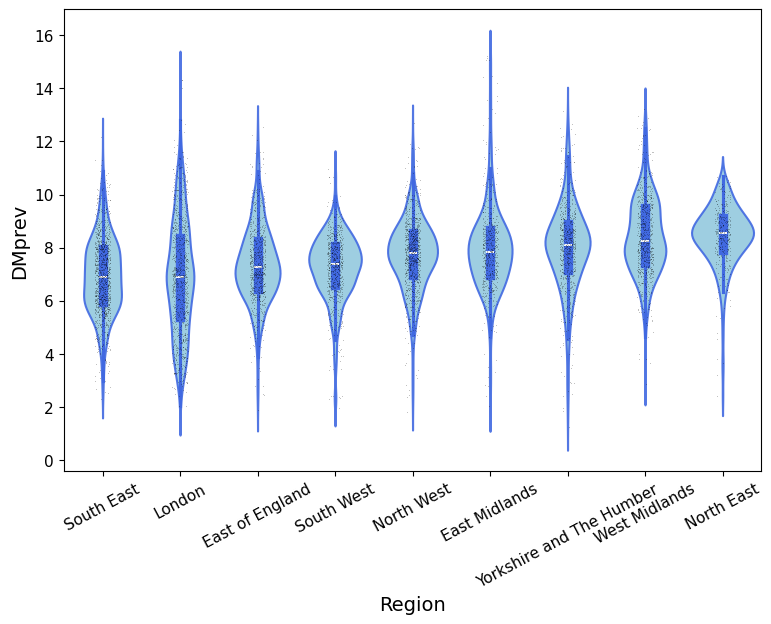
\includegraphics[width=1\linewidth]{ucl-latex-thesis-templates-master/Image/datageo_violin_3.1.png}
  \caption{Regions and DM prevalence.}
  \label{fig:A4.11}
\end{subfigure}%
\begin{subfigure}{.50\textwidth}
  \centering
  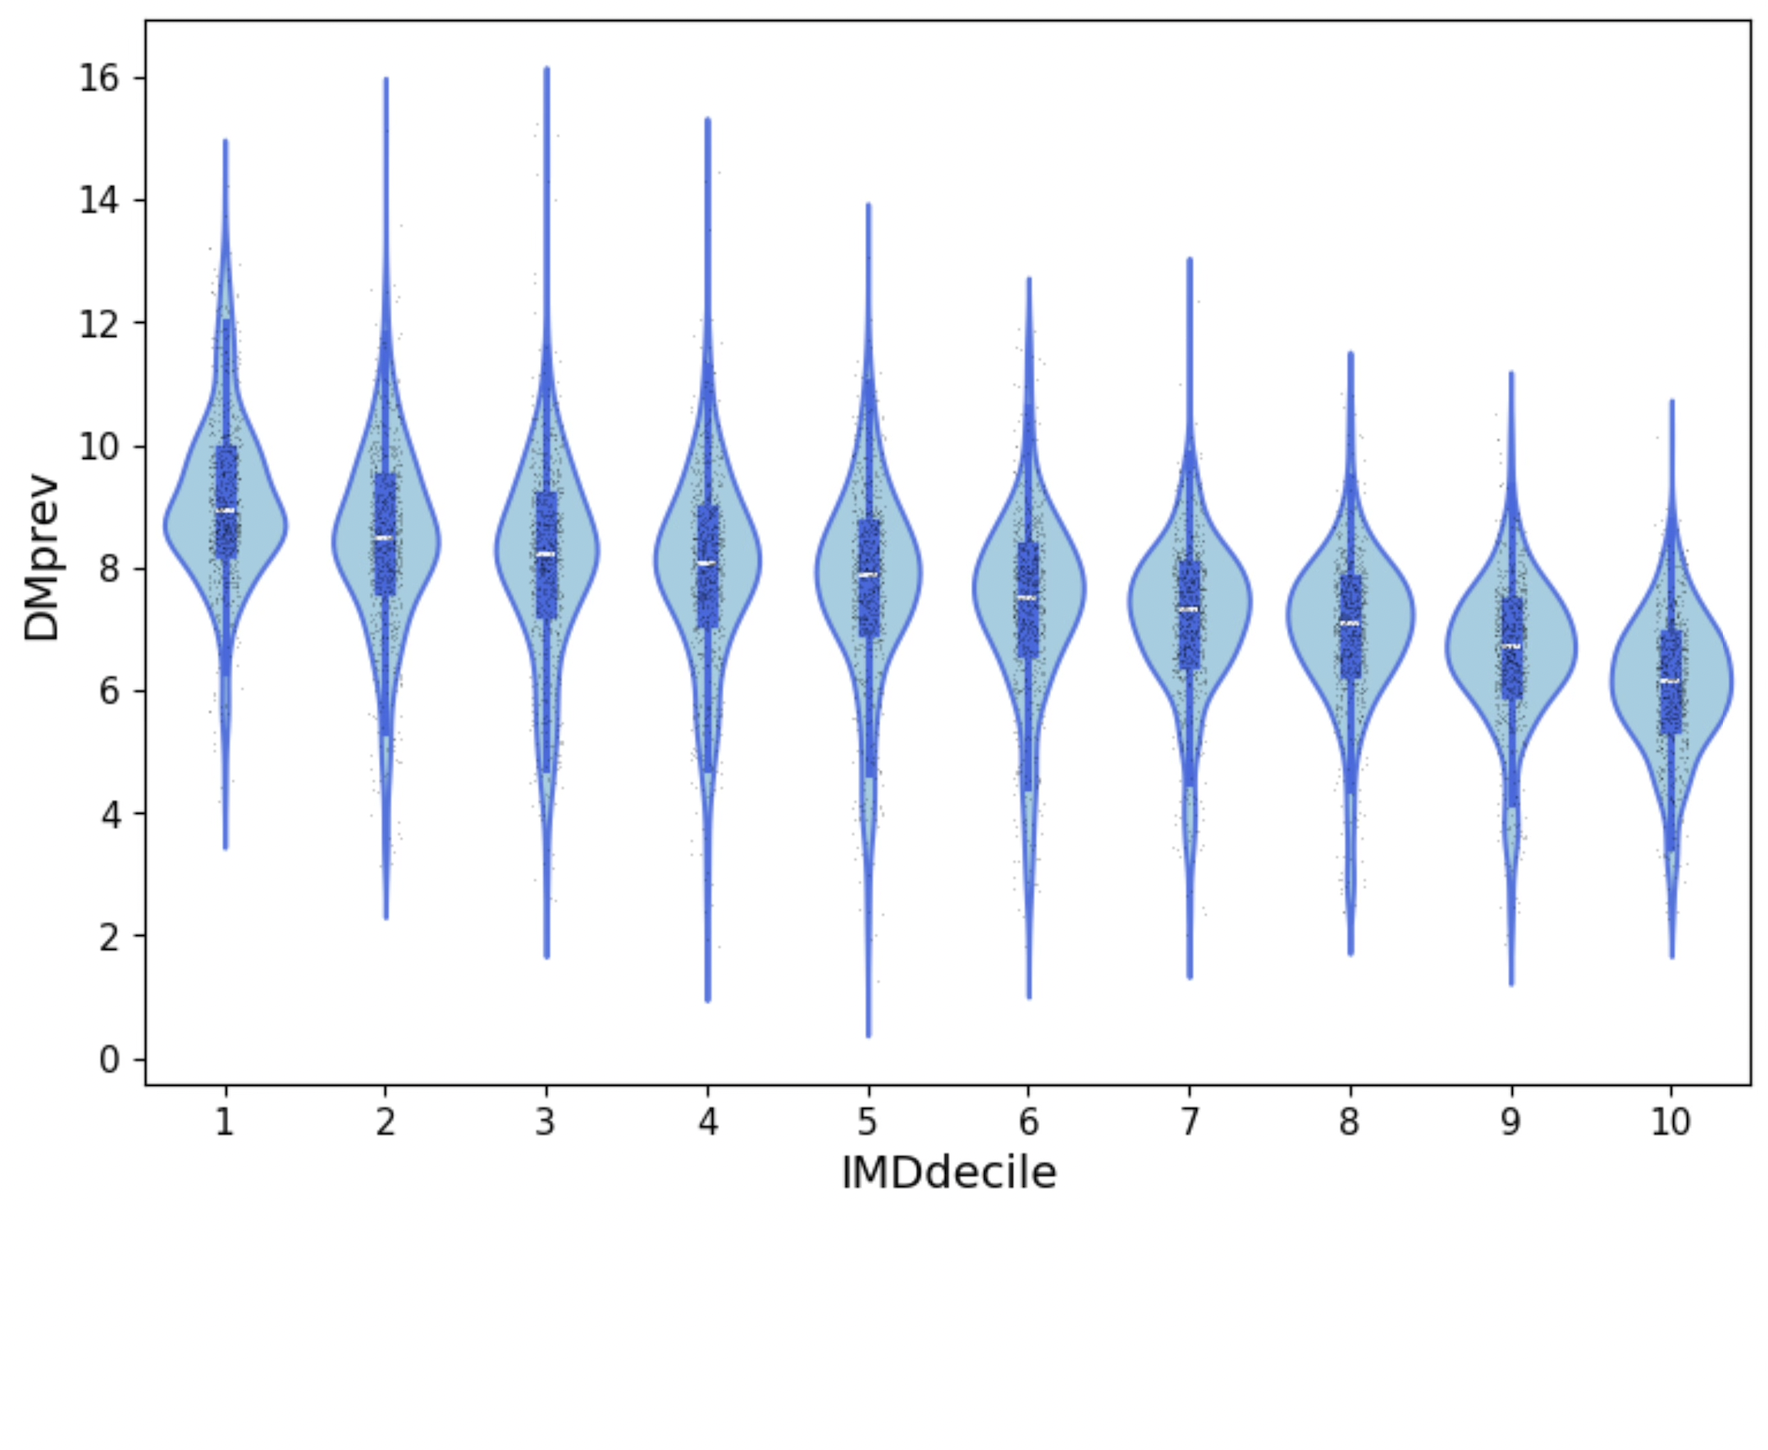
\includegraphics[width=1\linewidth]{ucl-latex-thesis-templates-master/Image/datageo_violin_3.2.png}
  \caption{IMD decile and DM prevalence.}
  \label{fig:A4.12}
\end{subfigure}
\caption{Violin plots for DM prevalence across nine regions and IMD deciles.}
\label{fig:A4.1}
\end{figure}

Figure \ref{fig:A4.2} shows the geographical distribution of DM prevalence. A Moran’s I statistic as high as 0.793 indicates a strong degree of spatial clustering. From the map, it’s evident that areas with very high DM prevalence are concentrated in the southern part of the North East, the eastern part of the East Midlands, and the northern part of the East of England. However, it’s interesting to note that despite this, the East of England has a median DM prevalence that ranks only the third-lowest out of the nine regions. We can also observe that cities like Oxford, Cambridge, and York have very low DM prevalence. In contrast, central England, including areas around cities like Birmingham, Nottingham, Sheffield, and Leeds, shows higher DM prevalence in the surrounding MSOAs.

Based on a review of the literature, I selected several risk factors that most scholars have emphasized, including obesity prevalence, IMD, and the Asian population, and mapped their geographical distribution (see Figure \ref{fig:A4.3}). We can see that the spatial distribution of obesity prevalence closely mirrors that of DM prevalence. IMD also shows a similar pattern, though to a slightly lesser extent. A common feature is that areas south of Grimsby exhibit both high DM and obesity prevalence, as well as high levels of deprivation. The Asian population, however, displays a different spatial pattern, concentrating around major cities. However, coincidentally, the MSOAs around these cities also tend to have a very high DM prevalence.


\begin{figure}[ht]
  \centering
  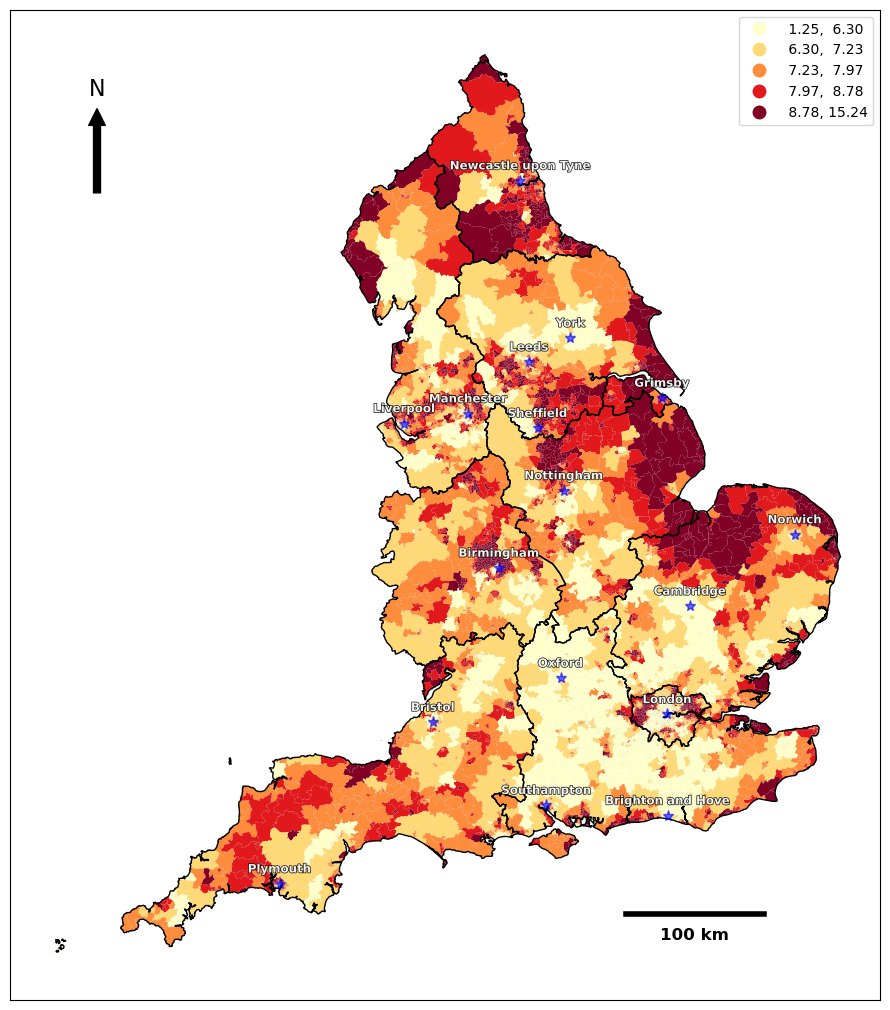
\includegraphics[width=.99\linewidth]{ucl-latex-thesis-templates-master/Image/datageo_DMprev_4.png}
  \caption{Geographical distribution of DM prevalence.}
  \label{fig:A4.2}
\end{figure}%


\begin{figure}[ht]
\centering
\begin{subfigure}{.4\textwidth}
  \centering
  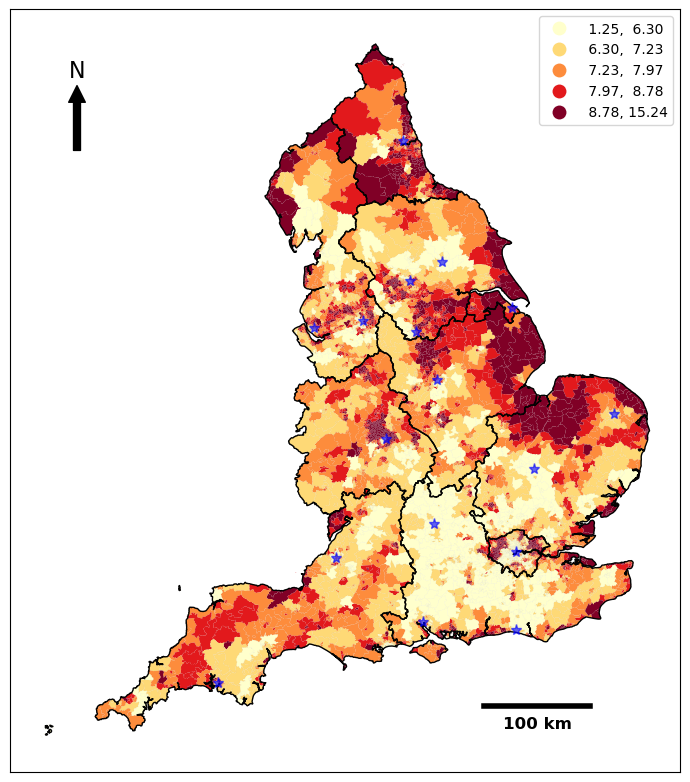
\includegraphics[width=1\linewidth]{ucl-latex-thesis-templates-master/Image/datageo_DMprev_5.png}
  \caption{DM prevalence.}
  \label{fig:A4.31}
\end{subfigure}%
\begin{subfigure}{.4\textwidth}
  \centering
  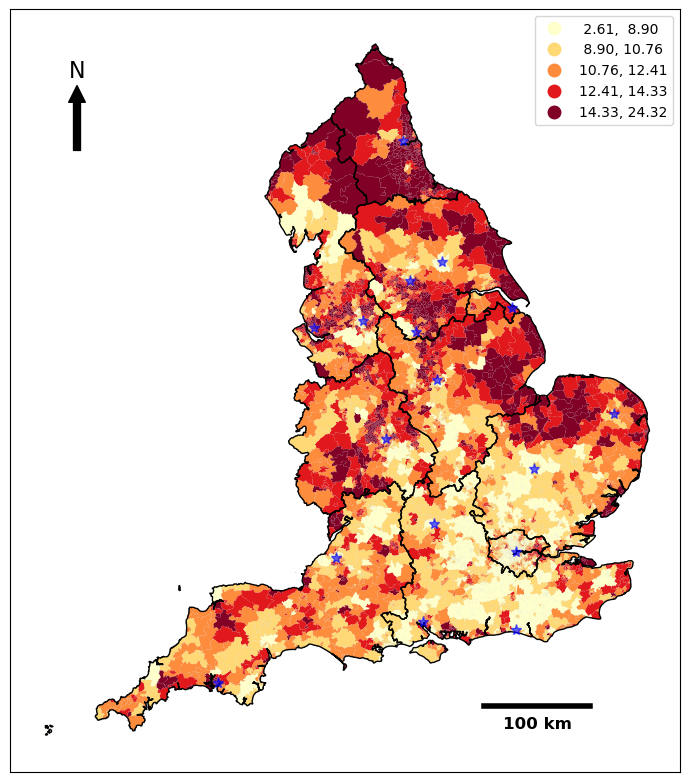
\includegraphics[width=1\linewidth]{ucl-latex-thesis-templates-master/Image/datageo_OBprev_6.png}
  \caption{Obesity prevalence.}
  \label{fig:A4.32}
\end{subfigure}
\begin{subfigure}{.4\textwidth}
  \centering
  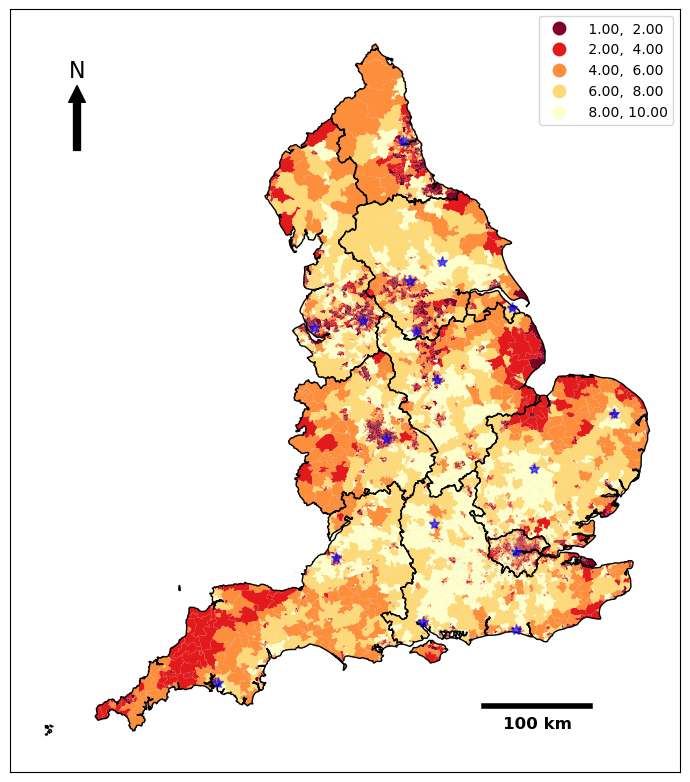
\includegraphics[width=1\linewidth]{ucl-latex-thesis-templates-master/Image/datageo_IMDdecile_7.png}
  \caption{IMD.}
  \label{fig:A4.33}
\end{subfigure}
\begin{subfigure}{.4\textwidth}
  \centering
  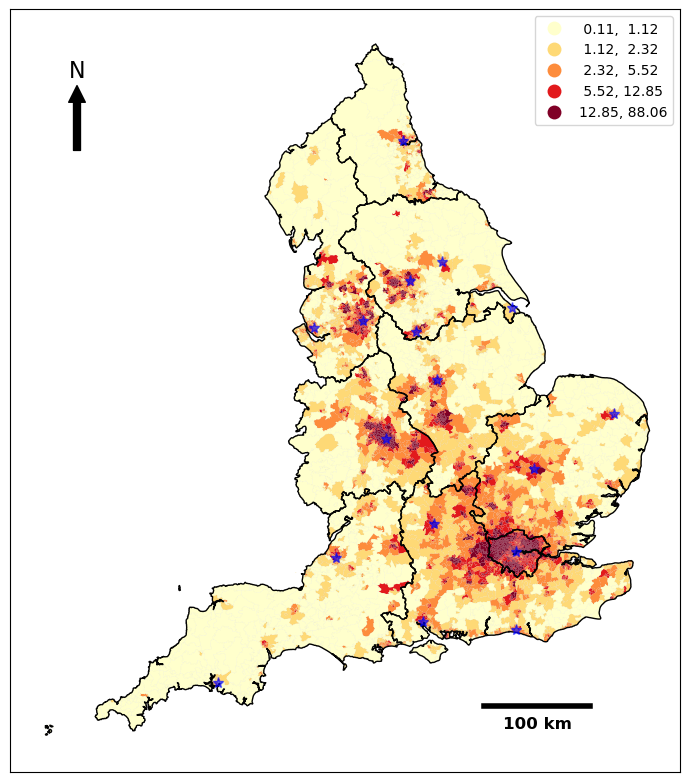
\includegraphics[width=1\linewidth]{ucl-latex-thesis-templates-master/Image/datageo_Asian_8.png}
  \caption{Asian population.}
  \label{fig:A4.34}
\end{subfigure}
\caption{Maps of selected variables.}
\label{fig:A4.3}
\end{figure}

\clearpage
\section{Correlation Analysis}
\label{chap:4.2}
Figure \ref{fig:A4.4} presents the correlation scatter plots between all independent variables and DM prevalence. Given the large number of observations, all independent variables show a significant correlation with DM prevalence, meaning no variables were eliminated at this stage. Among the ethnic groups, we observe a moderate positive correlation between the Asian population and DM prevalence, while Mixed, White, and Other populations all show a negative correlation with DM prevalence. Age17\_29 exhibits a clear negative linear relationship in the age groups, whereas Age60\_69 shows a positive linear relationship. Lifestyle factors and childcare are also positively correlated with DM prevalence, except for HighSSB. Figure \ref{fig:A4.5} displays the heat map of the correlation matrix, revealing what appears to be high multicollinearity among the independent variables.

\begin{figure}[ht]
  \centering
  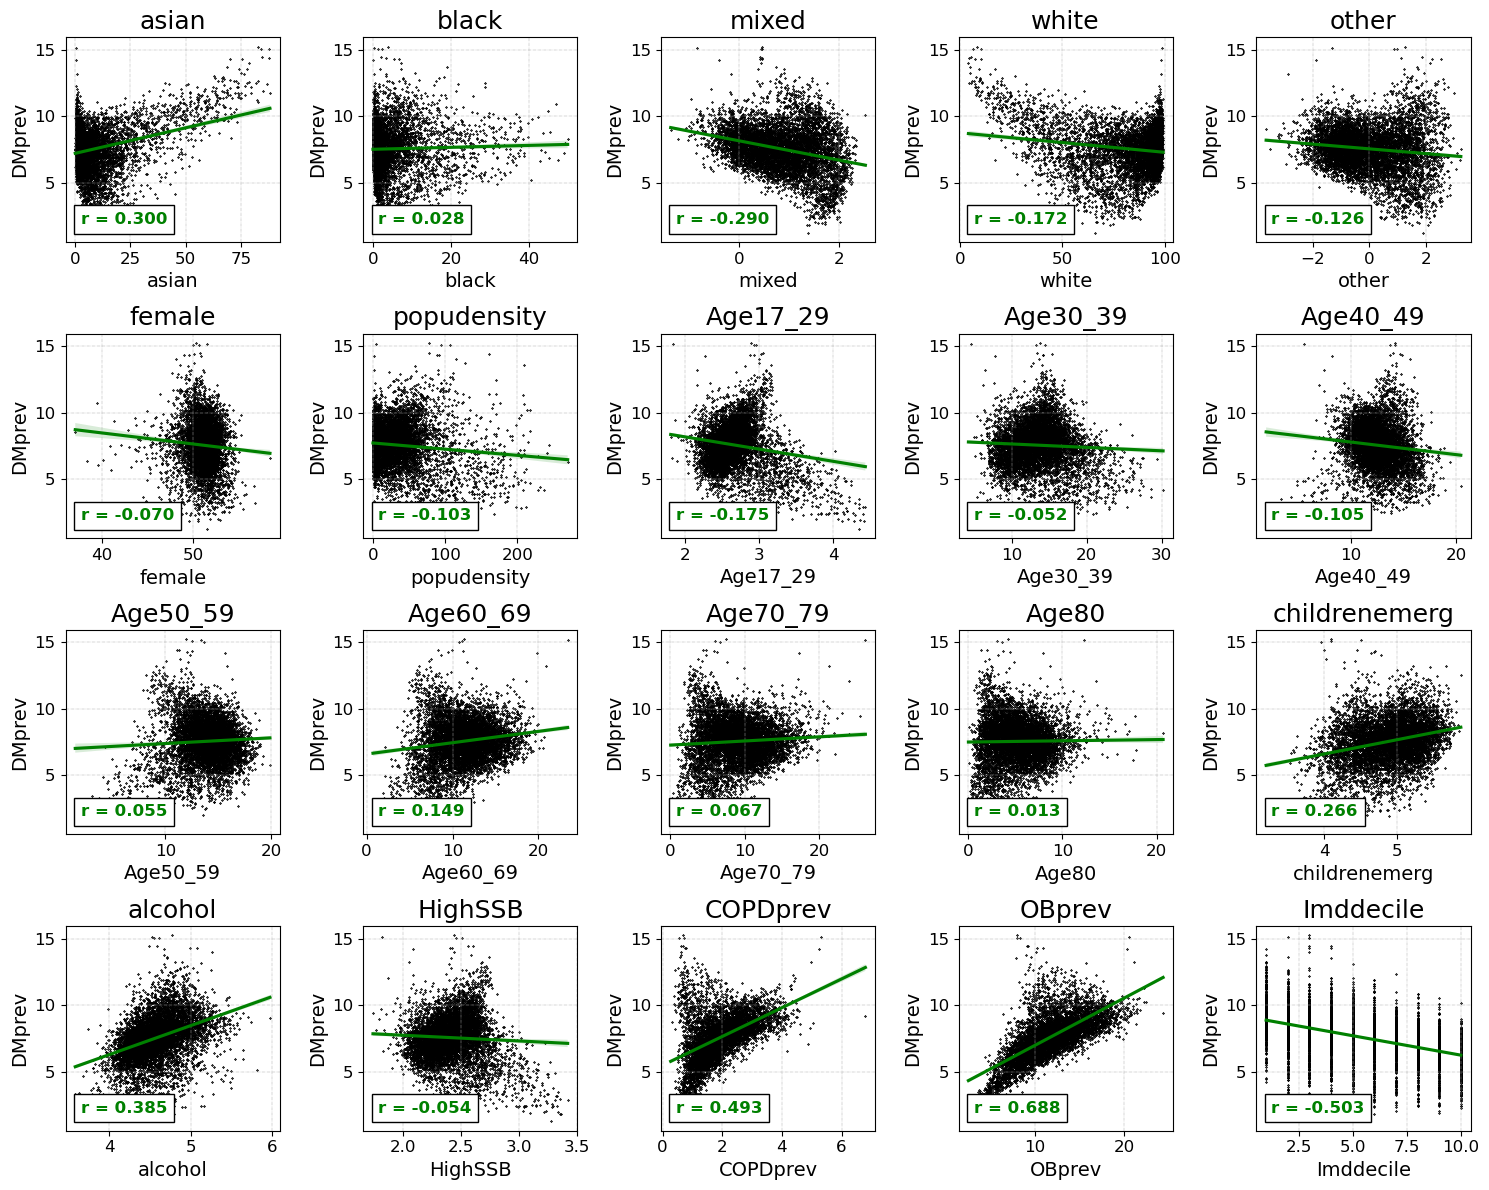
\includegraphics[width=.99\linewidth]{ucl-latex-thesis-templates-master/Image/methods_corrscat_1.png}
  \caption{Scatter plots of DM prevalence vs all explanatory variables.}
  \label{fig:A4.4}
\end{figure}%

\vspace{10pt}

\begin{figure}[ht]
  \centering
  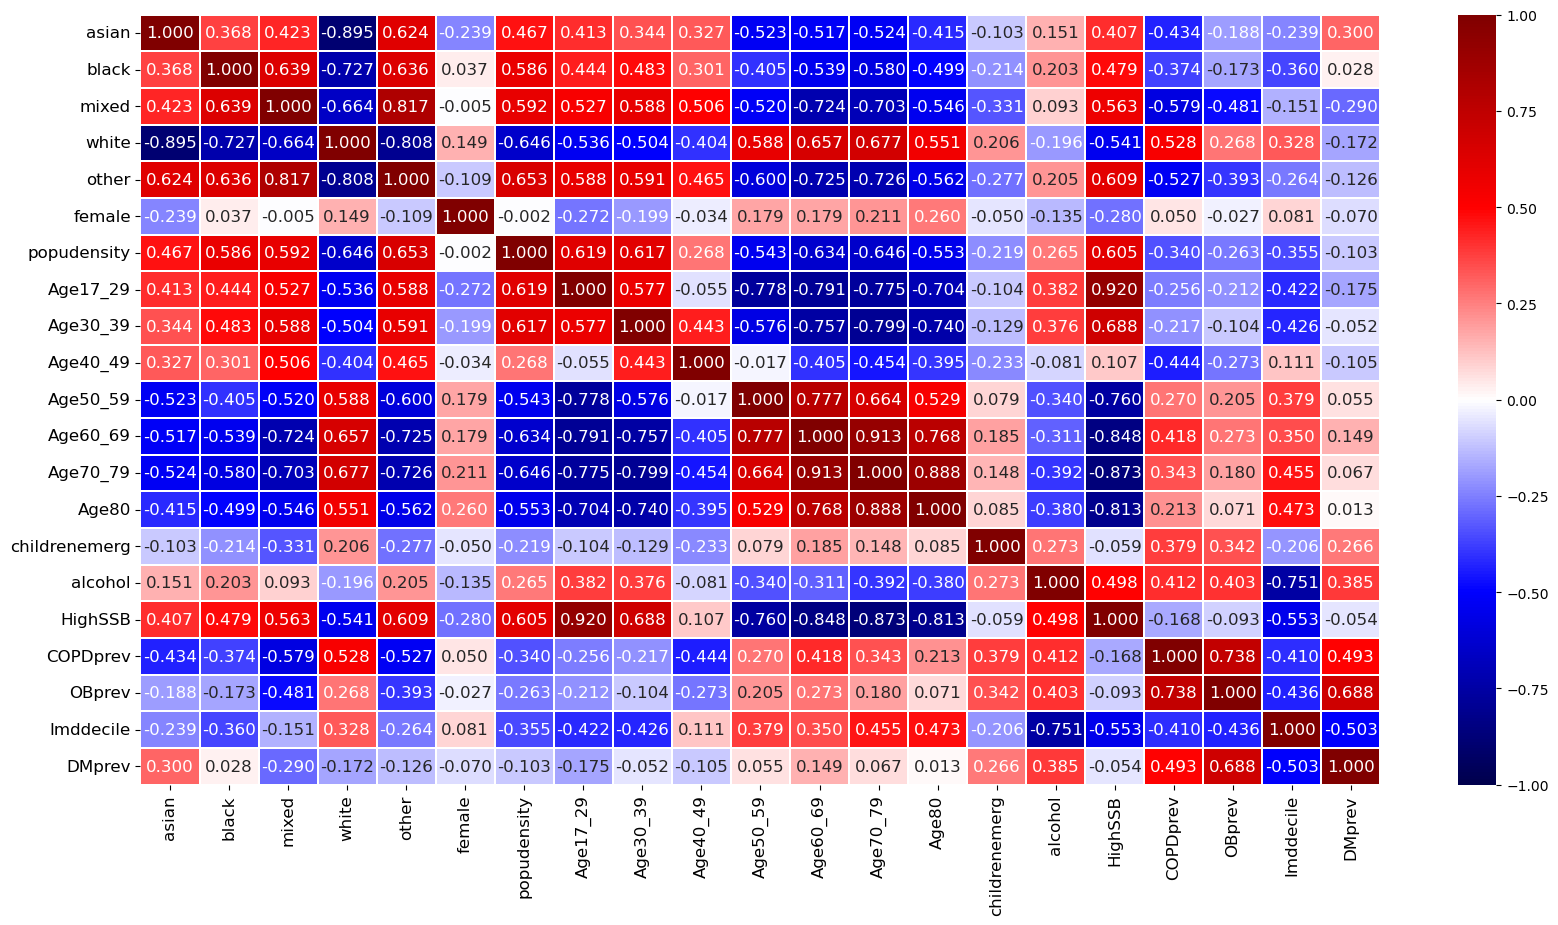
\includegraphics[width=.99\linewidth]{ucl-latex-thesis-templates-master/Image/methods_corrmatrix_2.png}
  \caption{Heat map of the correlation matrix.}
  \label{fig:A4.5}
\end{figure}%



\section{Ordinary Least Squares}
\label{chap:4.3}
We manually removed the two most prevalent variables from the age and ethnicity groups, Age17\_29 and White population, to avoid multicollinearity.
Table \ref{tab: A4.1} presents our initial OLS model based on a selection criterion of VIF < 4. Among the remaining variables, only Age30\_39, Children care, and Alcohol are not significant, while the others are significant. Since the data has been standardized, the coefficients can be compared. The top three contributing factors are the Asian population, obesity prevalence, and IMD decile. With an R-squared of 0.7613, the model demonstrates strong explanatory power, indicating that the independent variables account for 76.13\% of the variation in DM prevalence.
Table \ref{tab: A4.2} presents the OLS model after Backward Elimination, with a slight reduction in AIC without significantly affecting the R-squared. This suggests that Backward Elimination successfully removed the three non-significant variables, reducing model complexity without compromising its explanatory capacity.
Although the Jarque-Bera test's p-value is highly significant, indicating that the residuals of the model do not meet the assumption of normality due to the large number of observations, the Central Limit Theorem applies, allowing us to relax this assumption. Figure \ref{fig:A4.6} shows that, despite the significance of the Jarque-Bera test, the histogram of the residuals still largely follows a normal distribution, as expected under the Central Limit Theorem.
Table \ref{tab: A4.3} highlights that the residuals of the OLS model exhibit significant spatial autocorrelation, with a high Moran's I statistic of 0.573, indicating the need for spatial regression models. The LM diagnostics results shown in Table \ref{tab: A4.4} indicate that both the LM Lag and LM Error tests are significant. Additionally, the Robust LM tests for both models are also significant. Although the Robust LM Error statistic is larger (1674.75) than the Robust LM Lag (487.13), suggesting the use of an SEM, the significance of both statistics means that a more comprehensive SDM should also be considered.

%%%%%%%
%%%%%%% OLS VIF
%%%%%%%
\begin{table}[]
\centering
\begin{tabular}{|llllll|}
\hline
\multicolumn{1}{|l|}{\textbf{Variable}} & \multicolumn{1}{l|}{\textbf{Coefficient}} & \multicolumn{1}{l|}{\textbf{Std. Error}} & \multicolumn{1}{l|}{\textbf{P-value}} & \multicolumn{1}{l|}{\textbf{Significance}} & \textbf{VIF} \\ \hline
\multicolumn{1}{|l|}{(Intercept)}       & \multicolumn{1}{l|}{1.250e-15}            & \multicolumn{1}{l|}{0.005935}                    & \multicolumn{1}{l|}{1.00000}          & \multicolumn{1}{l|}{}                      & /            \\ \hline
\multicolumn{1}{|l|}{Asian}             & \multicolumn{1}{l|}{0.5560}               & \multicolumn{1}{l|}{0.008316}                    & \multicolumn{1}{l|}{\textless 2e-16}  & \multicolumn{1}{l|}{***}                   & 1.963303     \\ \hline
\multicolumn{1}{|l|}{Black}             & \multicolumn{1}{l|}{0.1228}               & \multicolumn{1}{l|}{0.008653}                    & \multicolumn{1}{l|}{\textless 2e-16}  & \multicolumn{1}{l|}{***}                   & 2.125326     \\ \hline
\multicolumn{1}{|l|}{Mixed}             & \multicolumn{1}{l|}{-0.1612}              & \multicolumn{1}{l|}{0.01100}                    & \multicolumn{1}{l|}{\textless 2e-16}  & \multicolumn{1}{l|}{***}                   & 3.434716     \\ \hline
\multicolumn{1}{|l|}{Female}            & \multicolumn{1}{l|}{0.0238}               & \multicolumn{1}{l|}{0.006665}                    & \multicolumn{1}{l|}{0.00036}          & \multicolumn{1}{l|}{***}                   & 1.260857     \\ \hline
\multicolumn{1}{|l|}{Popudensity}       & \multicolumn{1}{l|}{-0.1470}              & \multicolumn{1}{l|}{0.009263}                    & \multicolumn{1}{l|}{\textless 2e-16}  & \multicolumn{1}{l|}{***}                   & 2.435609     \\ \hline
\multicolumn{1}{|l|}{Age30\_39}         & \multicolumn{1}{l|}{0.01117}              & \multicolumn{1}{l|}{0.01119}                    & \multicolumn{1}{l|}{0.31801}          & \multicolumn{1}{l|}{}                      & 3.554550     \\ \hline
\multicolumn{1}{|l|}{Age40\_49}         & \multicolumn{1}{l|}{0.05527}              & \multicolumn{1}{l|}{0.009273}                    & \multicolumn{1}{l|}{2.64e-09}         & \multicolumn{1}{l|}{***}                   & 2.440698     \\ \hline
\multicolumn{1}{|l|}{Age50\_59}         & \multicolumn{1}{l|}{0.1439}               & \multicolumn{1}{l|}{0.009989}                    & \multicolumn{1}{l|}{\textless 2e-16}  & \multicolumn{1}{l|}{***}                   & 2.832384     \\ \hline
\multicolumn{1}{|l|}{Age80}             & \multicolumn{1}{l|}{0.2001}               & \multicolumn{1}{l|}{0.01001}                    & \multicolumn{1}{l|}{\textless 2e-16}  & \multicolumn{1}{l|}{***}                   & 2.841857     \\ \hline
\multicolumn{1}{|l|}{Childrenemerg}     & \multicolumn{1}{l|}{0.002875}             & \multicolumn{1}{l|}{0.006747}                    & \multicolumn{1}{l|}{0.67000}          & \multicolumn{1}{l|}{}                      & 1.292357     \\ \hline
\multicolumn{1}{|l|}{Alcohol}           & \multicolumn{1}{l|}{0.004924}             & \multicolumn{1}{l|}{0.009511}                    & \multicolumn{1}{l|}{0.60470}          & \multicolumn{1}{l|}{}                      & 2.567739     \\ \hline
\multicolumn{1}{|l|}{OBprev}            & \multicolumn{1}{l|}{0.5276}               & \multicolumn{1}{l|}{0.008856}                    & \multicolumn{1}{l|}{\textless 2e-16}  & \multicolumn{1}{l|}{***}                   & 2.226523     \\ \hline
\multicolumn{1}{|l|}{IMDdecile}         & \multicolumn{1}{l|}{-0.3203}              & \multicolumn{1}{l|}{0.01126}                    & \multicolumn{1}{l|}{\textless 2e-16}  & \multicolumn{1}{l|}{***}                   & 3.597933     \\ \hline \hline
\multicolumn{6}{|l|}{\textbf{Multiple R-squared:} 0.7613}                                                                                                                                        \\ \hline
\multicolumn{6}{|l|}{\textbf{Adjusted R-squared:} 0.7608}                                                                                                                                        \\ \hline
\multicolumn{6}{|l|}{\textbf{F-statistic:} 1662.29}                                                                                                                                              \\ \hline
\multicolumn{6}{|l|}{\textbf{F-statistic p value:} \textless 2.2e-16}                                                                                                                            \\ \hline
\multicolumn{6}{|l|}{\textbf{Log-Likelihood:} -4771.83}                                                                                                                                          \\ \hline
\multicolumn{6}{|l|}{\textbf{AIC:} 9573.66}                                                                                                                                                      \\ \hline
\multicolumn{6}{|l|}{\textbf{BIC:} 9676.01}                                                                                                                                                      \\ \hline
\multicolumn{6}{|l|}{\textbf{RMSE:} 0.4886}                                                                                                                                                      \\ \hline \hline
\multicolumn{6}{|l|}{\textbf{Durbin-Watson test:} 1.0012}                                                                                                                                        \\ \hline
\multicolumn{6}{|l|}{\textbf{Jarque-Bera test p value:} \textless 2.2e-16}                                                                                                                       \\ \hline
\multicolumn{6}{|l|}{\textbf{Goldfeld-Quandt test p value:} 0.3094}                                                                                                                              \\ \hline \hline
\multicolumn{6}{|l|}{\textbf{Significance codes:} 0 ‘***’ 0.001 ‘**’ 0.01 ‘*’ 0.05 ‘.’ 0.1 ‘ ’ 1}                                                                                                \\ \hline
\end{tabular}
\caption{
The summary statistics of the initial OLS model.
}
\label{tab: A4.1}
\end{table}


%%%%%%%
%%%%%%% OLS Stepwise
%%%%%%%
\clearpage
\begin{table}[]
\centering
\begin{tabular}{|llllll|}
\hline
\multicolumn{1}{|l|}{\textbf{Variable}} & \multicolumn{1}{l|}{\textbf{Coefficient}} & \multicolumn{1}{l|}{\textbf{Std. Error}} & \multicolumn{1}{l|}{\textbf{P-value}} & \multicolumn{1}{l|}{\textbf{Significance}} & \textbf{VIF} \\ \hline
\multicolumn{1}{|l|}{(Intercept)}       & \multicolumn{1}{l|}{1.807e-15}            & \multicolumn{1}{l|}{0.005934} & \multicolumn{1}{l|}{1.00000}          & \multicolumn{1}{l|}{}                      & /            \\ \hline
\multicolumn{1}{|l|}{Asian}             & \multicolumn{1}{l|}{0.5529}               & \multicolumn{1}{l|}{0.007853} & \multicolumn{1}{l|}{\textless 2e-16}  & \multicolumn{1}{l|}{***}                   & 1.750827     \\ \hline
\multicolumn{1}{|l|}{Black}             & \multicolumn{1}{l|}{0.1216}               & \multicolumn{1}{l|}{0.008577} & \multicolumn{1}{l|}{\textless 2e-16}  & \multicolumn{1}{l|}{***}                   & 2.088520     \\ \hline
\multicolumn{1}{|l|}{Mixed}             & \multicolumn{1}{l|}{-0.1608}              & \multicolumn{1}{l|}{0.01086} & \multicolumn{1}{l|}{\textless 2e-16}  & \multicolumn{1}{l|}{***}                   & 3.348141     \\ \hline
\multicolumn{1}{|l|}{Female}            & \multicolumn{1}{l|}{0.02237}              & \multicolumn{1}{l|}{0.006552} & \multicolumn{1}{l|}{0.000643}         & \multicolumn{1}{l|}{***}                   & 1.218749     \\ \hline
\multicolumn{1}{|l|}{Popudensity}       & \multicolumn{1}{l|}{-0.1444}              & \multicolumn{1}{l|}{0.008799} & \multicolumn{1}{l|}{\textless 2e-16}  & \multicolumn{1}{l|}{***}                   & 2.198365     \\ \hline
\multicolumn{1}{|l|}{Age40\_49}         & \multicolumn{1}{l|}{0.05928}              & \multicolumn{1}{l|}{0.008464} & \multicolumn{1}{l|}{2.72e-12}         & \multicolumn{1}{l|}{***}                   & 2.034045     \\ \hline
\multicolumn{1}{|l|}{Age50\_59}         & \multicolumn{1}{l|}{0.1394}               & \multicolumn{1}{l|}{0.009205} & \multicolumn{1}{l|}{\textless 2e-16}  & \multicolumn{1}{l|}{***}                   & 2.405596     \\ \hline
\multicolumn{1}{|l|}{Age80}             & \multicolumn{1}{l|}{0.1969}               & \multicolumn{1}{l|}{0.009474} & \multicolumn{1}{l|}{\textless 2e-16}  & \multicolumn{1}{l|}{***}                   & 2.548242     \\ \hline
\multicolumn{1}{|l|}{OBprev}            & \multicolumn{1}{l|}{0.5293}               & \multicolumn{1}{l|}{0.008710} & \multicolumn{1}{l|}{\textless 2e-16}  & \multicolumn{1}{l|}{***}                   & 2.153809     \\ \hline
\multicolumn{1}{|l|}{IMDdecile}         & \multicolumn{1}{l|}{-0.3259}              & \multicolumn{1}{l|}{0.009265} & \multicolumn{1}{l|}{\textless 2e-16}  & \multicolumn{1}{l|}{***}                   & 2.437461     \\ \hline \hline
\multicolumn{6}{|l|}{\textbf{Multiple R-squared:} 0.7612}                                                                                                                                        \\ \hline
\multicolumn{6}{|l|}{\textbf{Adjusted R-squared:} 0.7609}                                                                                                                                        \\ \hline
\multicolumn{6}{|l|}{\textbf{F-statistic:} 2161.28}                                                                                                                                              \\ \hline
\multicolumn{6}{|l|}{\textbf{F-statistic p value:} \textless 2.2e-16}                                                                                                                            \\ \hline
\multicolumn{6}{|l|}{\textbf{Log-Likelihood:} -4772.61}                                                                                                                                          \\ \hline
\multicolumn{6}{|l|}{\textbf{AIC:} 9569.23}                                                                                                                                                      \\ \hline
\multicolumn{6}{|l|}{\textbf{BIC:} 9651.11}                                                                                                                                                      \\ \hline
\multicolumn{6}{|l|}{\textbf{RMSE:} 0.4886}                                                                                                                                                      \\ \hline \hline
\multicolumn{6}{|l|}{\textbf{Durbin-Watson test:} 1.0029}                                                                                                                                        \\ \hline
\multicolumn{6}{|l|}{\textbf{Jarque-Bera test p value:} \textless 2.2e-16}                                                                                                                       \\ \hline
\multicolumn{6}{|l|}{\textbf{Goldfeld-Quandt test p value:} 0.2254}                                                                                                                              \\ \hline \hline
\multicolumn{6}{|l|}{\textbf{Significance codes:} 0 ‘***’ 0.001 ‘**’ 0.01 ‘*’ 0.05 ‘.’ 0.1 ‘ ’ 1}                                                                                                \\ \hline
\end{tabular}
\caption{
The summary statistics of the OLS model (after Backward Elimination).
}
\label{tab: A4.2}
\end{table}

\begin{figure}[!ht]
\centering
\begin{subfigure}{.45\textwidth}
  \centering
  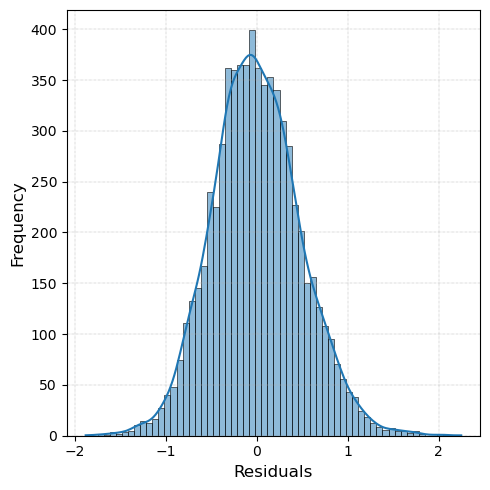
\includegraphics[width=1\linewidth]{ucl-latex-thesis-templates-master/Image/resi_OLS_1.1.png}
  \caption{Histogram.}
  \label{fig:A4.61}
\end{subfigure}%
\begin{subfigure}{.45\textwidth}
  \centering
  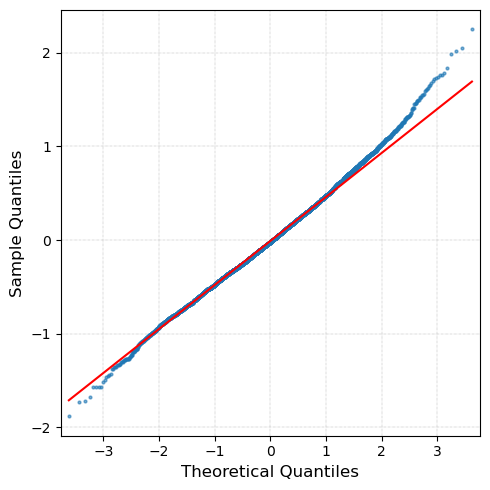
\includegraphics[width=1\linewidth]{ucl-latex-thesis-templates-master/Image/resi_OLS_1.2.png}
  \caption{Q-Q plot.}
  \label{fig:A4.62}
\end{subfigure}
\caption{OLS residuals analysis.}
\label{fig:A4.6}
\end{figure}

%%%%%%%
%%%%%%% Moran I test, LM Robust LM test
%%%%%%%
\begin{table}[]
\centering
\begin{tabular}{|l|l|l|}
\hline
\textbf{Data} & \textbf{Moran I statistic} & \textbf{P-value}  \\ \hline
DMprev        & 0.7931186                  & \textless 2.2e-16 \\ \hline
OLS Residuals & 0.5726112                  & \textless 2.2e-16 \\ \hline
\end{tabular}
\caption{
Moran I test for dependent variable and residuals of OLS model.
}
\label{tab: A4.3}
\end{table}


\begin{table}[]
\centering
\begin{tabular}{|l|l|l|l|}
\hline
\textbf{LM diagnostics} & \textbf{Statistic} & \textbf{P-value} & \textbf{Significance} \\ \hline
LM Lag                  & 4656.03            & \textless 2.2e-16 & ***                   \\ \hline
LM Error                & 5843.65            & \textless 2.2e-16 & ***                   \\ \hline
Robust LM Lag           & 487.13             & \textless 2.2e-16 & ***                   \\ \hline
Robust LM Error         & 1674.75            & \textless 2.2e-16 & ***                   \\ \hline \hline
\multicolumn{4}{|l|}{\textbf{Significance codes:} 0 ‘***’ 0.001 ‘**’ 0.01 ‘*’ 0.05 ‘.’ 0.1 ‘ ’ 1} \\ \hline
\end{tabular}
\caption{
LM diagnostics for spatial dependence
}
\label{tab: A4.4}
\end{table}


\section{Spatial Regression Analysis}
\label{chap:4.4}
Table \ref{tab: A4.5} presents the results of the SLM. We find that the value of Rho is 0.659, indicating a strong spatial dependence in DM prevalence. This means that when DM prevalence in neighboring areas increases by one standard deviation, the DM prevalence in the current area will increase by 0.659 standard deviations. Using Monte Carlo simulations, we calculated the direct effect, indirect effect, and total effect for each variable (see Table \ref{tab: A4.6}). The top three factors with the strongest total effect remain the Asian population, obesity prevalence, and IMD decile. Table \ref{tab: A4.7} presents the results of the SEM. We observe that the lambda value is as high as 0.899, suggesting a strong spatial autocorrelation in the error terms. This indicates that we may have omitted some spatial factors, resulting in spatial dependence that cannot be fully captured by the current independent variables.
Table \ref{tab: A4.8} shows the results of the SDM. Since the SDM is more complex than the SLM, and the regression coefficients for the independent variables cannot be directly compared or interpreted, it is essential to calculate the direct, indirect, and total effects for each variable. Based on Table \ref{tab: A4.9}, using the Asian variable as an example, when the Asian population in the current area increases by one standard deviation compared to the White population, the DM prevalence in the current area will increase by 0.294 standard deviations. When the Asian population in neighboring areas increases by one standard deviation compared to the White population, the DM prevalence in the current area will increase by 0.584 standard deviations. We can see that the top three factors in terms of total effect have shifted to the Asian population, IMD decile, and Age 80+. Obesity prevalence has fallen out of the top three because its indirect effect is not significant, meaning that obesity prevalence in neighboring areas does not have a significant impact on DM prevalence in the current area. We find that the Asian population, IMD decile, and advancing age exhibit strong spatial spillover effects, with their indirect effects exceeding their direct effects.

%%%%%%%
%%%%%%% SLM Table
%%%%%%%
\begin{table}[]
\centering
\begin{tabular}{|lllll|}
\hline
\multicolumn{1}{|l|}{\textbf{Variable}} & \multicolumn{1}{l|}{\textbf{Coefficient}} & \multicolumn{1}{l|}{\textbf{Std. Error}} & \multicolumn{1}{l|}{\textbf{P-value}}  & \textbf{Significance} \\ \hline
\multicolumn{1}{|l|}{(Intercept)}       & \multicolumn{1}{l|}{0.0172885}            & \multicolumn{1}{l|}{0.0039840}           & \multicolumn{1}{l|}{1.428e-05}         & ***                   \\ \hline
\multicolumn{1}{|l|}{Asian}             & \multicolumn{1}{l|}{0.2310246}            & \multicolumn{1}{l|}{0.0062791}           & \multicolumn{1}{l|}{\textless 2.2e-16} & ***                   \\ \hline
\multicolumn{1}{|l|}{Black}             & \multicolumn{1}{l|}{0.0471533}            & \multicolumn{1}{l|}{0.0058128}           & \multicolumn{1}{l|}{4.441e-16}         & ***                   \\ \hline
\multicolumn{1}{|l|}{Mixed}             & \multicolumn{1}{l|}{-0.0640843}           & \multicolumn{1}{l|}{0.0074030}           & \multicolumn{1}{l|}{\textless 2.2e-16} & ***                   \\ \hline
\multicolumn{1}{|l|}{Female}            & \multicolumn{1}{l|}{0.0268484}            & \multicolumn{1}{l|}{0.0043926}           & \multicolumn{1}{l|}{9.829e-10}         & ***                   \\ \hline
\multicolumn{1}{|l|}{Popudensity}       & \multicolumn{1}{l|}{-0.0436492}           & \multicolumn{1}{l|}{0.0059291}           & \multicolumn{1}{l|}{1.814e-13}         & ***                   \\ \hline
\multicolumn{1}{|l|}{Age40\_49}         & \multicolumn{1}{l|}{0.0662121}            & \multicolumn{1}{l|}{0.0056748}           & \multicolumn{1}{l|}{\textless 2.2e-16} & ***                   \\ \hline
\multicolumn{1}{|l|}{Age50\_59}         & \multicolumn{1}{l|}{0.0658630}            & \multicolumn{1}{l|}{0.0062171}           & \multicolumn{1}{l|}{\textless 2.2e-16} & ***                   \\ \hline
\multicolumn{1}{|l|}{Age80}             & \multicolumn{1}{l|}{0.1277811}            & \multicolumn{1}{l|}{0.0063836}           & \multicolumn{1}{l|}{\textless 2.2e-16} & ***                   \\ \hline
\multicolumn{1}{|l|}{OBprev}            & \multicolumn{1}{l|}{0.2281244}            & \multicolumn{1}{l|}{0.0070629}           & \multicolumn{1}{l|}{\textless 2.2e-16} & ***                   \\ \hline
\multicolumn{1}{|l|}{IMDdecile}         & \multicolumn{1}{l|}{-0.2179904}           & \multicolumn{1}{l|}{0.0063877}           & \multicolumn{1}{l|}{\textless 2.2e-16} & ***                   \\ \hline \hline
\multicolumn{1}{|l|}{\textbf{Rho}}               & \multicolumn{1}{l|}{0.65885}              & \multicolumn{1}{l|}{0.0073056}           & \multicolumn{1}{l|}{\textless 2.2e-16} & ***                   \\ \hline \hline
\multicolumn{5}{|l|}{\textbf{Wald statistic:} 8133.1, p-value: \textless 2.22e-16}                                                                                                                       \\ \hline
\multicolumn{5}{|l|}{\textbf{LR test value:} 4741.1, p-value: \textless 2.22e-16}                                                                                                                        \\ \hline
\multicolumn{5}{|l|}{\textbf{Log likelihood:} -2402.065}                                                                                                                                                 \\ \hline
\multicolumn{5}{|l|}{\textbf{AIC:} 4830.13}                                                                                                                                                              \\ \hline
\multicolumn{5}{|l|}{\textbf{BIC:} 4918.834}                                                                                                                                                             \\ \hline \hline
\multicolumn{5}{|l|}{\textbf{Significance codes:} 0 ‘***’ 0.001 ‘**’ 0.01 ‘*’ 0.05 ‘.’ 0.1 ‘ ’ 1}                                                                                                        \\ \hline
\end{tabular}
\caption{
The summary statistics of the SLM.
}
\label{tab: A4.5}
\end{table}


%%%%%%% SLM Impact
\begin{table}[]
\centering
\begin{tabular}{|l||l|l||l|l||l|l|}
\hline
\textbf{Variable} & \multicolumn{2}{c||}{\textbf{Direct}} & \multicolumn{2}{c||}{\textbf{Indirect}} & \multicolumn{2}{c|}{\textbf{Total}} \\ \hline
                  & \textbf{Value} & \textbf{p-value} & \textbf{Value} & \textbf{p-value} & \textbf{Value} & \textbf{p-value} \\ \hline
Asian             & 0.259 & \textless 2.22e-16 & 0.418 & \textless 2.22e-16 & 0.677 & \textless 2.22e-16 \\ \hline
Black             & 0.053 & 2.220e-16 & 0.085 & 2.220e-16 & 0.138 & 2.220e-16 \\ \hline
Mixed             & -0.072 & \textless 2.22e-16 & -0.116 & \textless 2.22e-16 & -0.188 & \textless 2.22e-16 \\ \hline
Female            & 0.030 & 1.346e-09 & 0.049 & 2.047e-09 & 0.079 & 1.510e-09 \\ \hline
Popudensity       & -0.049 & 3.175e-13 & -0.079 & 3.824e-13 & -0.128 & 2.645e-13 \\ \hline
Age40\_49         & 0.074 & \textless 2.22e-16 & 0.120 & \textless 2.22e-16 & 0.194 & \textless 2.22e-16 \\ \hline
Age50\_59         & 0.074 & \textless 2.22e-16 & 0.119 & \textless 2.22e-16 & 0.193 & \textless 2.22e-16 \\ \hline
Age80             & 0.143 & \textless 2.22e-16 & 0.231 & \textless 2.22e-16 & 0.375 & \textless 2.22e-16 \\ \hline
OBprev            & 0.256 & \textless 2.22e-16 & 0.413 & \textless 2.22e-16 & 0.669 & \textless 2.22e-16 \\ \hline
IMDdecile         & -0.245 & \textless 2.22e-16 & -0.394 & \textless 2.22e-16 & -0.639 & \textless 2.22e-16 \\ \hline
\end{tabular}
\caption{
Impact measures and simulated p-values for spatial lag model
}
\label{tab: A4.6}
\end{table}


%%%%%%%
%%%%%%% SEM Table
%%%%%%%
\begin{table}[]
\centering
\begin{tabular}{|lllll|}
\hline
\multicolumn{1}{|l|}{\textbf{Variable}} & \multicolumn{1}{l|}{\textbf{Coefficient}} & \multicolumn{1}{l|}{\textbf{Std. Error}} & \multicolumn{1}{l|}{\textbf{P-value}}  & \textbf{Significance} \\ \hline
\multicolumn{1}{|l|}{(Intercept)}       & \multicolumn{1}{l|}{0.0744906}            & \multicolumn{1}{l|}{0.0334254}           & \multicolumn{1}{l|}{0.0258431}         & *                     \\ \hline
\multicolumn{1}{|l|}{Asian}             & \multicolumn{1}{l|}{0.2810473}            & \multicolumn{1}{l|}{0.0086039}           & \multicolumn{1}{l|}{\textless 2.2e-16} & ***                   \\ \hline
\multicolumn{1}{|l|}{Black}             & \multicolumn{1}{l|}{0.1046913}            & \multicolumn{1}{l|}{0.0088935}           & \multicolumn{1}{l|}{\textless 2.2e-16} & ***                   \\ \hline
\multicolumn{1}{|l|}{Mixed}             & \multicolumn{1}{l|}{-0.1326065}           & \multicolumn{1}{l|}{0.0106191}           & \multicolumn{1}{l|}{\textless 2.2e-16} & ***                   \\ \hline
\multicolumn{1}{|l|}{Female}            & \multicolumn{1}{l|}{0.0154181}            & \multicolumn{1}{l|}{0.0039673}           & \multicolumn{1}{l|}{0.0001018}         & ***                   \\ \hline
\multicolumn{1}{|l|}{Popudensity}       & \multicolumn{1}{l|}{0.0209477}            & \multicolumn{1}{l|}{0.0072549}           & \multicolumn{1}{l|}{0.0038843}         & **                    \\ \hline
\multicolumn{1}{|l|}{Age40\_49}         & \multicolumn{1}{l|}{0.0554306}            & \multicolumn{1}{l|}{0.0060371}           & \multicolumn{1}{l|}{\textless 2.2e-16} & ***                   \\ \hline
\multicolumn{1}{|l|}{Age50\_59}         & \multicolumn{1}{l|}{0.0535536}            & \multicolumn{1}{l|}{0.0058865}           & \multicolumn{1}{l|}{\textless 2.2e-16} & ***                   \\ \hline
\multicolumn{1}{|l|}{Age80}             & \multicolumn{1}{l|}{0.1033838}            & \multicolumn{1}{l|}{0.0058598}           & \multicolumn{1}{l|}{\textless 2.2e-16} & ***                   \\ \hline
\multicolumn{1}{|l|}{OBprev}            & \multicolumn{1}{l|}{0.4645399}            & \multicolumn{1}{l|}{0.0088284}           & \multicolumn{1}{l|}{\textless 2.2e-16} & ***                   \\ \hline
\multicolumn{1}{|l|}{IMDdecile}         & \multicolumn{1}{l|}{-0.2295011}           & \multicolumn{1}{l|}{0.0064026}           & \multicolumn{1}{l|}{\textless 2.2e-16} & ***                   \\ \hline \hline
\multicolumn{1}{|l|}{\textbf{Lambda}}            & \multicolumn{1}{l|}{0.8988}              & \multicolumn{1}{l|}{0.0054564}           & \multicolumn{1}{l|}{\textless 2.2e-16} & ***                   \\ \hline \hline
\multicolumn{5}{|l|}{\textbf{Wald statistic:} 27134, p-value: \textless 2.22e-16}                                                                                                                        \\ \hline
\multicolumn{5}{|l|}{\textbf{LR test value:} 6064, p-value: \textless 2.22e-16}                                                                                                                     \\ \hline
\multicolumn{5}{|l|}{\textbf{Log likelihood:} -1740.616}                                                                                                                                              \\ \hline
\multicolumn{5}{|l|}{\textbf{AIC:} 3507.232}                                                                                                                                                             \\ \hline
\multicolumn{5}{|l|}{\textbf{BIC:} 3595.936}                                                                                                                                                           \\ \hline \hline
\multicolumn{5}{|l|}{\textbf{Significance codes:} 0 ‘***’ 0.001 ‘**’ 0.01 ‘*’ 0.05 ‘.’ 0.1 ‘ ’ 1}                                                                                                      \\ \hline
\end{tabular}
\caption{
The summary statistics of the SEM.
}
\label{tab: A4.7}
\end{table}

%%%%%%%
%%%%%%% SDM Table
%%%%%%%
\begin{table}[]
\centering
\begin{tabular}{|l|l|l|l|l|}
\hline
\textbf{Variable} & \textbf{Coefficient} & \textbf{Std. Error} & \textbf{P-value} & \textbf{Significance} \\ \hline
(Intercept)       & 0.0035706            & 0.0034390           & 0.2991453        &                       \\ \hline
Asian             & 0.2593663            & 0.0090437           & \textless 2.2e-16 & ***                   \\ \hline
Black             & 0.1099056            & 0.0091326           & \textless 2.2e-16 & ***                   \\ \hline
Mixed             & -0.1166722           & 0.0107779           & \textless 2.2e-16 & ***                   \\ \hline
Female            & 0.0152904            & 0.0040001           & 0.0001321        & ***                   \\ \hline
Popudensity       & 0.0322634            & 0.0073054           & 1.004e-05        & ***                   \\ \hline
Age40\_49         & 0.0529707            & 0.0060282           & \textless 2.2e-16 & ***                   \\ \hline
Age50\_59         & 0.0580807            & 0.0059257           & \textless 2.2e-16 & ***                   \\ \hline
Age80             & 0.1071359            & 0.0058703           & \textless 2.2e-16 & ***                   \\ \hline
OBprev            & 0.4453933            & 0.0091057           & \textless 2.2e-16 & ***                   \\ \hline
IMDdecile         & -0.2324876           & 0.0063867           & \textless 2.2e-16 & ***                   \\ \hline \hline
\multicolumn{1}{|l|}{\textbf{Lagged Variable}} & \multicolumn{1}{l|}{\textbf{Coefficient}} & \multicolumn{1}{l|}{\textbf{Std. Error}} & \multicolumn{1}{l|}{\textbf{P-value}}  & \textbf{Significance} \\ \hline
lag.Asian         & -0.1125014           & 0.0121396           & \textless 2.2e-16 & ***                   \\ \hline
lag.Black         & -0.0810433           & 0.0113147           & 7.911e-13        & ***                   \\ \hline
lag.Mixed         & 0.0792986            & 0.0132281           & 2.038e-09        & ***                   \\ \hline
lag.Female        & -0.0021617           & 0.0071244           & 0.7615671        &                       \\ \hline
lag.Popudensity   & -0.0753573           & 0.0099948           & 4.707e-14        & ***                   \\ \hline
lag.Age40\_49     & -0.0372915           & 0.0092084           & 5.128e-05        & ***                   \\ \hline
lag.Age50\_59     & 0.0042647            & 0.0096405           & 0.6582224        &                       \\ \hline
lag.Age80         & -0.0302246           & 0.0106338           & 0.0044788        & **                    \\ \hline
lag.OBprev        & -0.3764927           & 0.0120199           & \textless 2.2e-16 & ***                   \\ \hline
lag.IMDdecile     & 0.1276194            & 0.0104037           & \textless 2.2e-16 & ***                   \\ \hline \hline
\textbf{Rho}              & 0.83342             & 0.0071322           & \textless 2.2e-16 & ***          \\ \hline \hline
\multicolumn{5}{|l|}{\textbf{Wald statistic:} 13655, p-value: \textless 2.22e-16} \\ \hline
\multicolumn{5}{|l|}{\textbf{LR test value:} 5487.5, p-value: \textless 2.22e-16} \\ \hline
\multicolumn{5}{|l|}{\textbf{Log likelihood:} -1508.157} \\ \hline
\multicolumn{5}{|l|}{\textbf{AIC:} 3062.313} \\ \hline
\multicolumn{5}{|l|}{\textbf{BIC:} 3219.25} \\ \hline \hline
\multicolumn{5}{|l|}{\textbf{Significance codes:} 0 ‘***’ 0.001 ‘**’ 0.01 ‘*’ 0.05 ‘.’ 0.1 ‘ ’ 1} \\ \hline
\end{tabular}
\caption{
The summary statistics of the SDM.
}
\label{tab: A4.8}
\end{table}

%%%%%%% SDM Impact
\begin{table}[]
\centering
\begin{tabular}{|l||l|l||l|l||l|l|}
\hline
\textbf{Variable} & \multicolumn{2}{c||}{\textbf{Direct}} & \multicolumn{2}{c||}{\textbf{Indirect}} & \multicolumn{2}{c|}{\textbf{Total}} \\ \hline
                  & \textbf{Value} & \textbf{p-value} & \textbf{Value} & \textbf{p-value} & \textbf{Value} & \textbf{p-value} \\ \hline
Asian             & 0.294 & \textless 2.22e-16 & 0.584 & \textless 2.22e-16 & 0.877 & \textless 2.22e-16 \\ \hline
Black             & 0.114 & \textless 2.22e-16 & 0.059 & 0.111543 & 0.173 & 4.6444e-06 \\ \hline
Mixed             & -0.123 & \textless 2.22e-16 & -0.101 & 0.034351 & -0.223 & 8.3267e-06 \\ \hline
Female            & 0.019 & 9.2171e-05 & 0.060 & 0.109482 & 0.078 & 0.052492 \\ \hline
Popudensity       & 0.016 & 0.037328 & -0.273 & 1.2919e-11 & -0.257 & 1.5203e-09 \\ \hline
Age40\_49         & 0.055 & \textless 2.22e-16 & 0.038 & 0.358950 & 0.093 & 0.037407 \\ \hline
Age50\_59         & 0.076 & \textless 2.22e-16 & 0.297 & 1.4185e-09 & 0.373 & 1.2721e-12 \\ \hline
Age80             & 0.127 & \textless 2.22e-16 & 0.333 & 8.1217e-10 & 0.460 & 2.2204e-15 \\ \hline
OBprev            & 0.444 & \textless 2.22e-16 & -0.032 & 0.382130 & 0.412 & \textless 2.22e-16 \\ \hline
IMDdecile         & -0.255 & \textless 2.22e-16 & -0.372 & 1.3323e-14 & -0.627 & \textless 2.22e-16 \\ \hline
\end{tabular}
\caption{
Impact measures and simulated p-values for SDM
}
\label{tab: A4.9}
\end{table}

\clearpage
\section{Model Selection and Comparison}
\label{chap:4.5}

Table \ref{tab: A4.10} presents the results of the LR test comparing the SDM with the SLM and SEM. We found that both sets of test statistics are very large, and the p-values are significant, indicating that the SDM cannot be simplified to either the SLM or SEM. Additionally, the AIC values for the SLM, SEM, and SDM are 4830.13, 3507.232, and 3062.313, respectively. Their BIC values are 4918.834, 3595.936, and 3219.25, respectively. Therefore, both the AIC and BIC show that the SDM has the lowest values, suggesting that it provides the best fit.
Figure \ref{fig:A4.7} shows the residuals maps of the four regression models we tested. It is clear that the residuals from the OLS model exhibit significant spatial autocorrelation, with most areas of underestimation showing spatial clustering. The SLM reduces some of the spatial autocorrelation, but Moran's I remains significant. The SEM and SDM successfully capture and address the spatial autocorrelation in the data, with Moran's I statistics of 0.01 (p-value greater than 0.05). Given that the SDM provides the best fit and successfully eliminates the spatial autocorrelation in the residuals, and considering Turi's (2017) discussion on spatial spillover effects, the SDM is compelling. Therefore, we have chosen the SDM as our final model.






%%%%%%% SDM LM test for degradation
\begin{table}[]
\centering
\begin{tabular}{|l|l|l|l|}
\hline
\textbf{LR test} & \textbf{Statistic} & \textbf{P-value} & \textbf{Significance} \\ \hline
SDM SLM                  & 1787.82            & \textless 2.2e-16 & ***                   \\ \hline
SDM SEM                & 464.92            & \textless 2.2e-16 & ***                   \\ \hline \hline
\multicolumn{4}{|l|}{\textbf{Significance codes:} 0 ‘***’ 0.001 ‘**’ 0.01 ‘*’ 0.05 ‘.’ 0.1 ‘ ’ 1} \\ \hline
\end{tabular}
\caption{
SDM LR test for degradation
}
\label{tab: A4.10}
\end{table}



\clearpage
\begin{figure}[ht]
\centering
\begin{subfigure}{.4\textwidth}
  \centering
  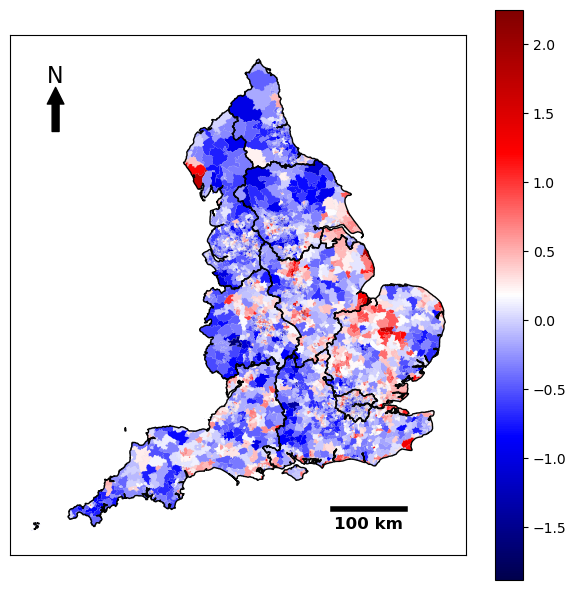
\includegraphics[width=1\linewidth]{ucl-latex-thesis-templates-master/Image/resi_OLS_1.png}
  \caption{OLS.}
  \label{fig:A4.71}
\end{subfigure}%
\begin{subfigure}{.4\textwidth}
  \centering
  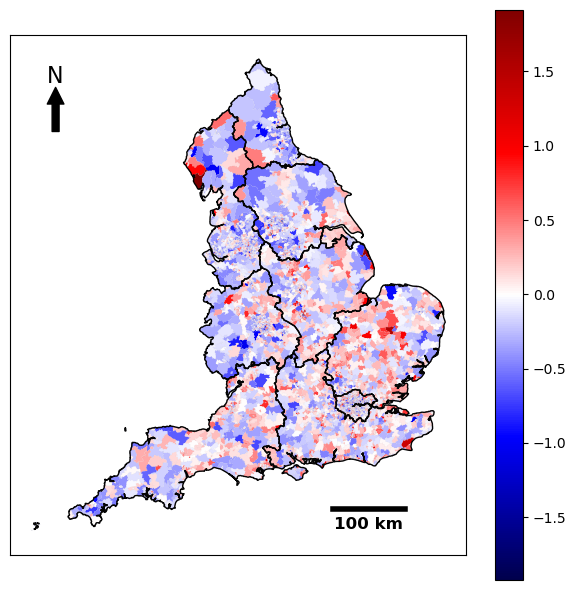
\includegraphics[width=1\linewidth]{ucl-latex-thesis-templates-master/Image/resi_SLM_2.png}
  \caption{SLM.}
  \label{fig:A4.72}
\end{subfigure}
\begin{subfigure}{.4\textwidth}
  \centering
  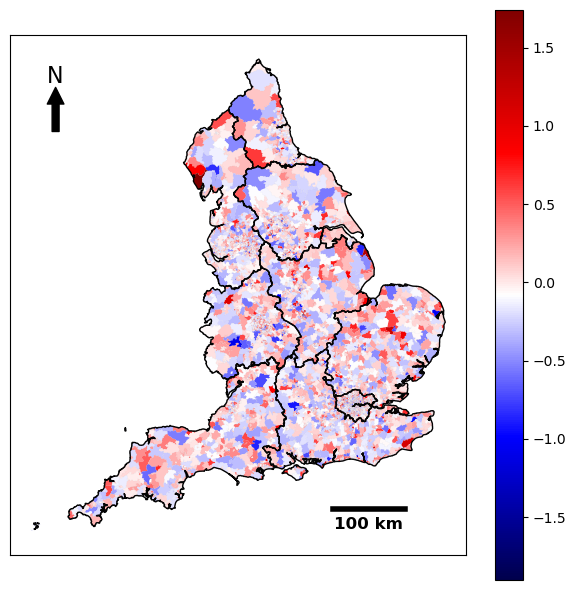
\includegraphics[width=1\linewidth]{ucl-latex-thesis-templates-master/Image/resi_SEM_3.png}
  \caption{SEM.}
  \label{fig:A4.73}
\end{subfigure}
\begin{subfigure}{.4\textwidth}
  \centering
  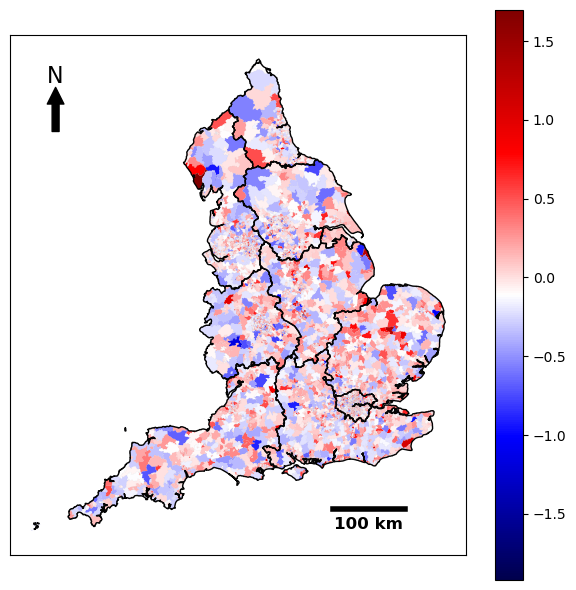
\includegraphics[width=1\linewidth]{ucl-latex-thesis-templates-master/Image/resi_SDM_4.png}
  \caption{SDM.}
  \label{fig:A4.74}
\end{subfigure}
\caption{Residual Maps for each regression model.}
\label{fig:A4.7}
\end{figure}